\chapter{Methodology}
\label{cap:method}

\intro{Introduction}\\

In this chapter, we will present the methodology used to develop the proposed solution. The chapter is divided into two sections: architecture, and implementation. The architecture section will present the proposed solution's architecture for the chosen cloud providers, while the implementation section will detail the steps taken to implement the solution.

\section{Architecture}

\begin{figure}[htbp]
    \centering
    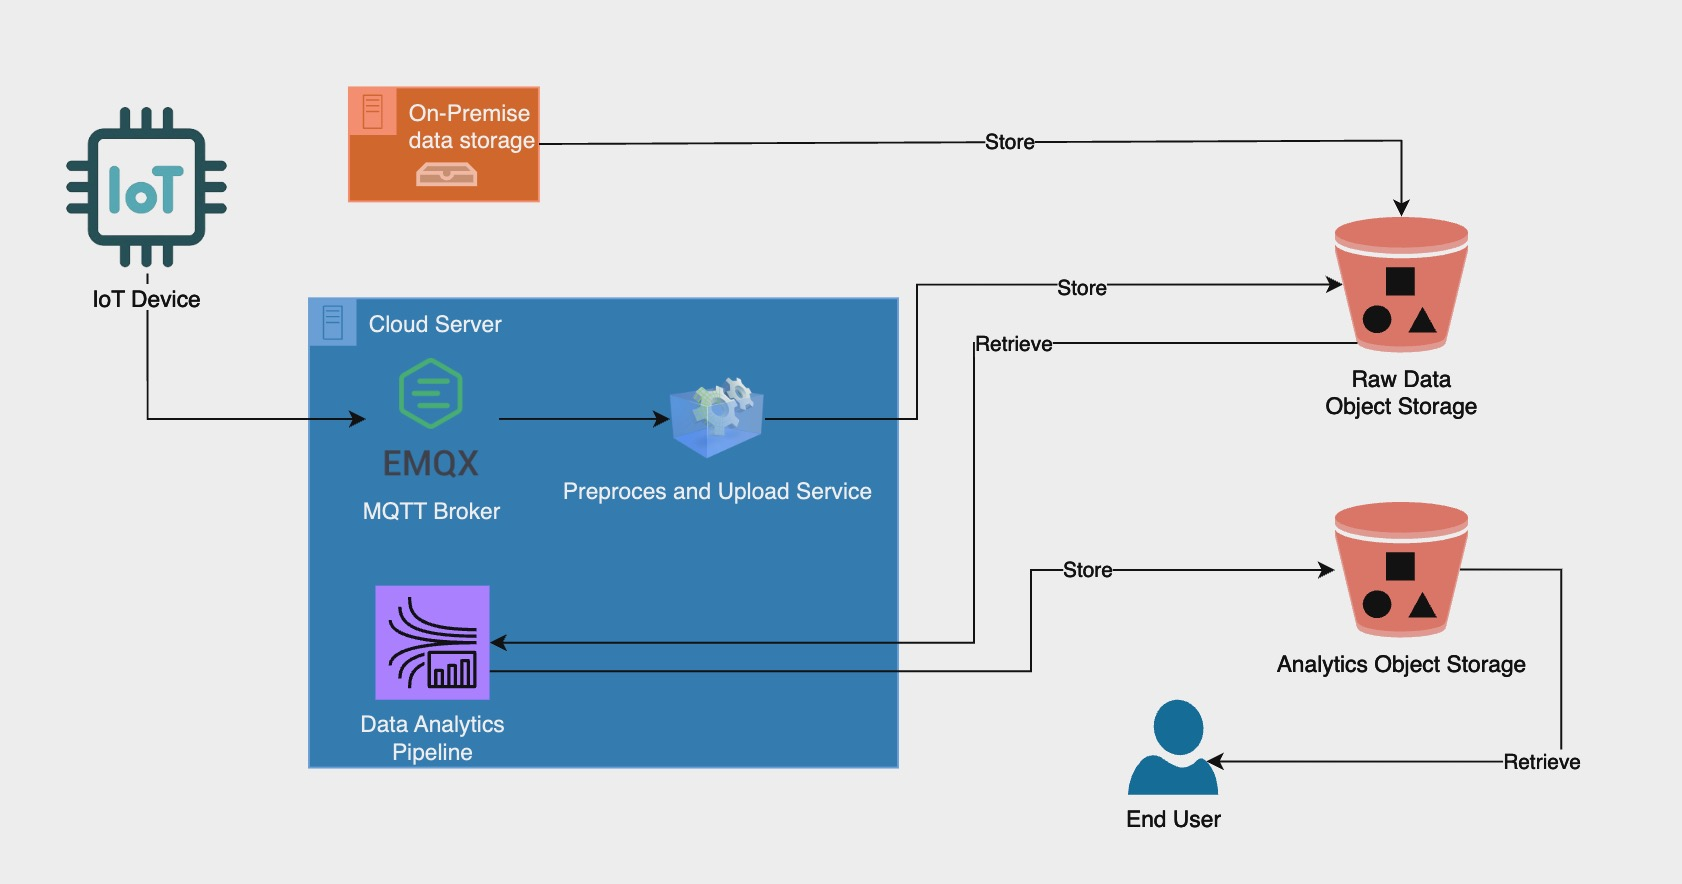
\includegraphics[width=1\textwidth]{architecture.png}
    \caption{Architecture of the proposed solution}
\end{figure}

The proposed solution's architecture consists of a composition of loosely coupled microservices that work together to collect, process, and store data. The architecture is divided into three layers: the data collection layer, the data storage layer and the data analysis layer. Each layer plays a specific role in the overall system, ensuring scalability, flexibility, and resilience.

\subsection{Data Collection Layer}

The data collection layer is responsible for gathering data from IoT devices and archived data. 

\subsection{Data Collection from IoT Devices}

The data collection from IoT devices utilizes the MQTT protocol, a lightweight messaging protocol designed for devices with low bandwidth and high latency. MQTT operates on a publish-subscribe model, where devices publish messages to a broker, which then forwards the messages to subscribers. This protocol is ideal for IoT devices due to its simplicity, ease of implementation, and reliability, with support for different quality of service (QoS) levels to ensure message delivery.

In our scenario, a large number of IoT devices publish data to the cloud. Each device publishes data to a specific topic managed by a cloud-based broker. The data is sent in JSON format, with each message containing a timestamp and a set of key-value pairs representing the data. Once the data is published to the broker, it undergoes preprocessing before being stored in object storage. This preprocessing involves parsing the JSON data, extracting the timestamp and key-value pairs, and converting the data to CSV format, which is less verbose than JSON. The preprocessed data is then stored in object storage, making it accessible to the data processing pipeline.


\subsection{Data Collection from Archived Data}
The data collection from archived data is done by uploading files from on-premises to the cloud via a simple script that leverages cloud API. The files, which are already in CSV format, are uploaded to the object storage, where they can be accessed by the data processing pipeline. The files contain historical data that have been collected over time in a number of different scenarios.

\subsection{Data Storage Layer}

The data storage layer is responsible for storing the raw CSV data and making it accessible to the data processing pipeline. This layer utilizes cloud-based object storage for scalability and durability. The data, always stored in CSV format, is uploaded to the object storage by the data collection layer and accessed by the data analysis layer.
Once the analysis is done, the results are stored in a separate object storage bucket, making them accessible to other services or users.
The object storage provides a reliable and cost-effective solution for storing large amounts of data, with built-in redundancy and scalability features.

\subsection{Data Analysis Layer}

The data analysis layer is responsible for analyzing the collected data and generating insights. This layer consists of several services that retrieve the preprocessed data from the object storage and perform various analytical tasks. The data, initially preprocessed and stored in CSV format, is accessed directly from the object storage by the microservices.

Once the data is retrieved, the microservices perform advanced analytics and machine learning tasks using custom algorithms tailored to specific requirements. These analytical processes transform the raw data into valuable insights, enabling more informed decision-making and deeper understanding of the underlying patterns and trends in the collected data.
Right after the analysis is done, the results are stored in a separate object storage bucket, making them accessible to other services or users.

\subsection{Cloud Server vs. SaaS Solutions}

The choice of using a cloud server to host both the MQTT broker and the data analytics pipeline provides several advantages over SaaS solutions. While SaaS architectures have been considered, a cloud server offers more flexibility and control over the infrastructure, which is crucial for custom configurations and dependencies required by the data analytics pipeline. It is also more cost-effective for long-term projects, as SaaS solutions typically incur significant monthly fees. A cloud server allows better control over costs, with the trade-off being the need to manage infrastructure and security patches.

Furthermore, this solution is seamlessly implementable with any cloud provider since it doesn't rely on specific services unique to a particular provider. This cloud-agnostic approach allows users to choose the cloud provider that best fits their needs without altering the solution's architecture. Additionally, even though the MQTT broker and the data analytics pipeline are hosted on the same server, they remain independent, respecting the principles of a microservices architecture.

In summary, this architecture provides a robust, scalable, and flexible solution for data collection, processing, and storage, with the added benefit of being cloud-agnostic and cost-effective for long-term deployments.

\section{Implementation}

The implementation of the proposed solution involves several steps, including setting up the cloud server, configuring the MQTT broker, setting up the storage services , and developing the data processing pipeline. The implementation is divided into two main components: the data collection component and the data analysis component.

\subsection{Data Collection Component}

The data collection component is responsible for collecting data from IoT devices and archived data. This component consists of two main parts: the MQTT broker and the data upload script.

\subsubsection{MQTT Broker}


\subsubsection{Data Upload Script}


\subsection{Data Analysis Component}

